\documentclass[12pt]{article}
\usepackage[utf8]{inputenc}
\usepackage[english]{babel}
\usepackage{array}
\usepackage{pdflscape}
\usepackage{amsthm,amsmath,icomma,amsfonts,amssymb,mathtools}
\mathtoolsset{showonlyrefs=true}
\usepackage{cmap}
\usepackage{booktabs}
\usepackage{graphicx}
%\usepackage[top = 25mm, bottom = 35mm, left = 30mm, right = 15mm]{geometry}
\usepackage[top = 25mm, bottom = 35mm, left = 23mm, right = 22mm]{geometry}
\usepackage{hyperref}
\usepackage[usenames,dvipsnames,svgnames,table,rgb]{xcolor}
\hypersetup{
	unicode = true,
	pdftitle = {Recursive Non-parametric Estimation of the Copula Density},
	pdfauthor = {Vladimir Yashin},
	pdfsubject = {Copula Density},
	pdfkeywords = {copula density} {recursive estimation} {statistics},
	colorlinks = true,
	linkcolor = blue,
	citecolor = blue,
	urlcolor = blue
}
\usepackage{tikz}

\newtheorem{theorem}{Theorem}
\newtheorem{remark}{Remark}

\usepackage[natbib=true,backend=biber,bibencoding=utf8,style=authoryear-comp,maxcitenames=2]{biblatex}
\addbibresource{library.bib}

\begin{document}
	%\maketitle
	\thispagestyle{empty}
	\newpage
	\begin{center}
		\textsc{
			federal state autonomous educational institution \\ 
			for higher professional education \\
			national research university higher school of economics \\
		}
		\textit{Faculty: St. Petersburg School of Economics and Management}
		\vspace*{\fill}
		
		Vladimir Yashin \\[1em]
		\textsc{Master Thesis} \\[1em]
		\textbf{RECURSIVE NON-PARAMETRIC ESTIMATION \\OF THE COPULA DENSITY} \\[1em]
		Field of study: 01.04.02 Applied Mathematics and Informatics\\[1em]
		Degree program: Big Data Analysis in Business, Economy, and Society
		
		\vspace*{\fill}
		
		\begin{tabular} {p{0.55\linewidth} p{0.55\linewidth}}
			Reviewer  & Supervisor \\[0.5em]
			\makebox[15em]{\hrulefill} & Assistant Professor, Ph.\,D.\\[0.5em]
			\makebox[15em]{\hrulefill} & Faculty of Computer Science \\[0.5em]
			\makebox[15em]{\hrulefill} & Geoffrey Decrouez \\[0.5em]
		\end{tabular}
		
		\vspace*{\fill}
		Saint Petersburg \\
		2018
	\end{center}
	\clearpage
	\newpage
	\noindent
	
	\begin{abstract}
		The contribution of this paper is two-fold. First of all, we introduced an algorithm that estimates the joint density function using the smoothed non-parametric recursive estimator. Secondly, for the first time, we present a smoothed non-parametric recursive estimator for a multivariate copula density, a joint distribution that can capture complex dependence structures among its variates. Also, we present the numerical results that show an apparent convergence of these estimators.\\
		\\
		\textbf{Key words}: stochastic approximation algorithms, on-line estimation, copula density.
	\end{abstract}
	
	\setcounter{page}{1}
	
	\section{Introduction}
	Two parts explain the nature of a random vector: (a) the marginal behaviour of each component; and (b) the dependence structure that governs the association between these components. Both can be achieved using copulas \parencite{Sklar1959}. Specifically, let $ \mathbf{X}=(X_1, \dots, X_d) \in \mathbb{R}^d $ be a random vector with joint cumulative distribution function $ F $ and its continuous marginals $ F_1, \dots, F_d $, given $ d \geq 2 $. The quantile of order $ u_j $ is defined as $ q^{u_j} := F^{-1}_j(u_j) $, for $ u_j\in(0, 1), ~j=1\dots d $. According to Sklar's theorem, the joint distribution of $ \mathbf{X} $ can be represented by means of a unique function $ C:(0, 1)^d \rightarrow(0, 1) $ such that
	\begin{align}
		C(u_1, \dots, u_d) = F\big(F^{-1}_1(u_1), \dots, F^{-1}_d(u_d)\big) = F\big(q^{u_1}, \dots, q^{u_d}\big). \label{eq:copula_def}
	\end{align}
	The function $ C $ is referred to as the copula. The proof of the existence of $ C $ was not been provided in \textcite{Sklar1959} but has been provided later on in \textcite{Moore1975} and \textcite{Deheuvels1978}.
	
	Copulas find several applications in many fields. First of all, use of copulas lies in finance and insurance risk management. The methodology that relies on the notion of the copulas was prevalent in finance in the early to mid 00's. Copulas are well suited for the field of financial markets as they are inherently volatile and erratic. 
	
	Some earlier applications involve modelling the default correlation between financial instruments. To measure the correlation, it is crucial to estimate the joint distribution for the survival times (time until default) of the instruments. The notion of copulas is quite useful in this case as they input marginal distributions that are generally can be derived from credit curves which are constructed using the information that is available on the market, and return the joint distribution of survival times \parencite{Li1999}. Other authors claim that the model must be dynamic, which requires measuring default risks of other obligors on a daily basis \parencite{Schonbucher2001}.
	
	Another group of authors aimed to find evidence of the dependence of credit risk in credit default swaps on stock performance. In particular, they were looking for tail dependence between markets. Since the marginal distributions are asymmetric and tail correlation is not linear, the copulas are used as they can capture non-linear relationship.  \parencite{Dupuis2009,DaSilva2014,Andersen2004,Kresta2012}. For a more comprehensive review of how copulas are applied in finance a reader is referred to \textcite{Cherubini2004}, \textcite{Patton2009}, and \textcite{Patton2012}.
	
	Besides, copulas are used in the fields of hydrology and climatology. Most hydrological events are multivariate. For example, climate events like storms and floods are usually described using several dependent random variables like volume, duration, peak etc. For more information of this application the reader is referred to \parencite{Favre2004,Genest2007,Renard2007,Chu2011,Dempster2007,Friedman2010,Piantadosi2012a,Piantadosi2012b,Salvadori2007}.
	
	Copulas also can be applied to sampling task including generation of stationary time-series. The main advantage of copulas in this regard is the fact that they are capable of accounting not only for correlations but also for the complete dependence structure, unlike other methods. See also \parencite{Strelen2009,Strelen2007,Erhardt2010,Erhardt2012,Nelsen2007,Matthias2017,Hyrs2015}.
	
	In this work, we introduce for the first time an algorithm of the estimation of a multivariate copula density function using joint distribution and marginal distribution functions. The joint and marginals, as well as the multivariate copula density, are estimated using the smoothing non-parametric recursive estimators.
	
	This paper is divided into seven sections. Section~2 presents the review of the traditional batch estimation of the copula. In the third section, the recursive estimate of the quantile can be found as well as a historical preview of this topic. Section~4, we introduce the recursive estimation of the copula density. Then, we discuss how to select a proper bandwidth for the presented algorithms. Section~6 presents the numerical results for a set of copulas with different parameter as well as the different choice of bandwidths.
	
	\section{Traditional Ways of Copula Estimation}\label{sec:traditional}
	
	In this section, we present a comprehensive review of the previously developed traditional batch-based methods of the copula estimation. 	
	
	Suppose that $ \mathbf{X}_1, \dots, \mathbf{X}_N $ is a sequence of i.i.d. random variables such that $ \mathbf{X}_i = (X_{i, 1}, \dots, X_{i, d}) \in \mathbb{R}^d $. The first non-parametric approach to estimate $ C $ was introduced in \textcite{Ruschendorf1976}, using pseudo-observations.
	
	Let $ C(u_1, \dots, u_d) $ be a copula and $ F $ is a cumulative distribution function, and $ F_1, \dots, F_d $ are its marginals
	\begin{align}
		C(u_1, \dots, u_d) &= F\big(F^{-1}_1(u_1), \dots, F^{-1}_d(u_d)\big) \\
		&\approx \frac{1}{n} \sum_{i=1}^{N} \mathbf{1}\big(X_{i, 1} \leq F_1^{-1}(u_1), \dots, X_{i, d} \leq F_d^{-1}(u_d)\big) \label{eq:copula_hat} \\
		&= \frac{1}{n} \sum_{i=1}^{N} \mathbf{1}\big(F_1(X_{i, 1}) \leq u_1, \dots, F_d(X_{i, d}) \leq u_d\big), 
	\end{align}
	where for each of the marginals $ F_j(X_{i, j}) ~ \forall j\in1\dots d $
	\begin{align}
		F_j(X_{i, j}) &= \mathbb{P}\big(\mathbf{X}_j \leq X_{i, j}\big)  \\
		&= \mathbb{P}\big((X_{i, 1}, \dots, X_{i, d}) \leq X_{i, j}\big) \\
		&\approx \frac{1}{n} \sum_{k=1}^{N} \mathbf{1}\big(X_{k, j} \leq X_{i, j}\big) \\
		&=: X^\star_{i, j}.
	\end{align}
	The variable $ X^\star_{i, j} $ represent the normalized rank of the $ j $-th element of the $ i $-th observation. Then, the copula estimator is
	\begin{align}
		\widehat{C}_n(\mathbf{u}) := \frac{1}{n}\sum_{i=1}^{N} \mathbf{1}\big(\mathbf{X}^\star_i \leq \mathbf{u}\big), 
	\end{align}
	where $ \mathbf{X}^\star_i = (X^\star_{i, 1}, \dots, X^\star_{i, d}) $ and $ \mathbf{u} = (u_1, \dots, u_d) $. Alternatively, a copula may be estimated using empirical quantiles \parencite{Deheuvels1979}. The empirical quintiles are usually defined as follows
	\begin{align}
	Q^{u_j}_n := \inf_\vartheta \Bigg\{ \frac{1}{n} \sum_{i=1}^{N} \mathbf{1}\big(X_{i, j} \leq \vartheta \big) \geq u_j \Bigg\}.
	\end{align}
	Then, given $ F_j^{-1}(u_j) = Q^{u_j}_n $ we may obtain from \eqref{eq:copula_hat} the estimator of copula which is simply
	\begin{align}
	\widetilde{C}_n (\mathbf{u}) := \frac{1}{n}\sum_{i=1}^{N} \mathbf{1}\big(\mathbf{X}_i \leq \mathbf{Q}^{\mathbf{u}}_n\big), 
	\end{align}
	where $ \mathbf{Q}^{\mathbf{u}}_n := (Q^{u_1}_n, \dots, Q^{u_d}_n) $.
		
	Both $ \widehat{C}_n $ and $ \widetilde{C}_n $ need to be completely recalculated once a new observation is obtained. This makes it essentially useless in practice since data flow can have a quite large $ N $. In this study, we purpose an on-line version of copula estimator that requires only $ \mathcal{O}(N) $ operations, i.\,e. making updates in $ \mathcal{O}(1) $ operations. This can be achieved using a recursive estimation of the quantiles.
	
	\section{Recursive Estimation of the Quantile}
	
	This section presents the perquisites of stochastic approximation methods as well as the application of this method specifically to the estimation of the quantile.
	
	In general, the task is to find the root of a function $ f: \mathbb{R} \rightarrow \mathbb{R} $. The first idea is to use the Newton's procedure that involve calculation of $ f $ at some point and a first-order derivative
	\begin{align}
		x_{n} = x_{n-1} - \frac{f(x_{n-1})}{f'(x_{n-1})}.
	\end{align}
	However, $ f $ is not necessarily differentiable. Thus, we may use a slightly less efficient algorithm which though addresses this issue. Generally it can be defined as follows
	\begin{align}
		x_n = x_{n-1} - \alpha f(x_{n-1}), \label{eq:for_robbins}
	\end{align}
	where $ \alpha $ is a positive number that defines a step size. Then, let us assume that we do not know the analytical expression for $ f $ and only have noisy observations $ f(x_n) + \varepsilon_n $ where $ \mathbb{E}[\varepsilon_n] = 0 $ for each $ n \in 1\dots N $. So, $ f(x_n) $ can be replaced by averaging many noisy observations such that
	\begin{align}
		f(x_n) &\approx \frac{1}{m} \sum_{i=1}^{m} \big(f(x_i)+\varepsilon_i\big) \\
		&\equiv \frac{1}{m} \sum_{i=1}^{m} F(x_i, \varepsilon_i).
	\end{align}
	Then, \eqref{eq:for_robbins} can be rewritten in the following way
	\begin{align}
		x_{n} = x_{n-1} - \frac{\alpha}{m}\sum_{i=1}^{m}F(x_i, \varepsilon_i).
	\end{align}
	
	Note that this algorithm is obviously inefficient as it is required to run it $ m $ times for every $ n $. To solve this problem, \textcite{Robbins1951} suggested to use the following
	\begin{align}
		x_n = x_{n-1} - \alpha_n F(x_n, \varepsilon_n), 
	\end{align}
	where $ \alpha_n $ is the sequence of positive numbers that converge to 0 such that $ \sum_n\alpha_n = \infty $ and $ \sum_n\alpha_n^2 < \infty $. Using the Robbins-Monro algorithm we can derive a recursive estimator of a quantile. 
	
	Let us take $ F\big(Q^{u_j}_n, X_{n, j}\big) = \mathbf{1} \big(X_{n, j} \leq Q^{u_j}_n\big) - u_j $ for $ u_j \in (0, 1) $, also consider a continuous function $ G $ such that $ G(Q^{u_j}_n) $ is well defined. Then, 
	\begin{align}
		f(x) &= \mathbb{E}\big[F(Q^{u_j}_n, X_{n, j})\big] \\
		&=\mathbb{P}\big(X_{n, j}\leq Q^{u_j}_n\big) - u_j \\
		&= G(Q^{u_j}_n) - u_j.
	\end{align}
	The root of this function is exactly $ u_j $ quantile of $ G $ and, thus, can be written recursively as
	\begin{align}
		Q^{u_j}_n = Q^{u_j}_{n-1} + \alpha_n \Big(u_j - \mathbf{1}\big(X_{n, j}\leq Q^{u_j}_{n-1}\big)\Big).
	\end{align}
	This estimator can be further applied for estimation of probability density function which is required in the recursive quantile estimator itself as well as in the copula density estimator. 
	
	The on-line estimation of a probability density were initially introduced in late 60's in \textcite{Wolverton1969} and studied in 70's by, for example, \textcite{Yamato1971}, \textcite{Davies1973}, \textcite{Wegman1979}. Later in late 00's similar results were presented from the view of stochastic approximation in \textcite{Mokkadem2009}; the application of the presented estimators was introduced in \textcite{Slaoui2014}.
	
	There two ways how to estimate a probability density function: parametric and non-parametric. The parametric approach relies on the idea that a random set of random variables $ X_1, \dots, X_N $ belongs a parametric family of distributions and these parameters can be estimated, for example, using maximum a posteriori hypothesis. Otherwise, the non-parametric approach has no assumptions regarding a distribution. 
	
	A non-parametric approach of the estimation of the quantile $ Q^{u_j}_n $ involves an indicator function, so that that the updates do not depend on how high the difference is. It does not matter how much the current estimation of the quantile is higher or lower than the current data point, the size of the increment will be the same. It is natural to introduce a kernel to address this issue \parencite{Amiri2014}. Though, for the simplicity, an indicator is used in this study.  We may rewrite and define an algorithm for estimation of empirical quantiles using on-line updates as follows
	\begin{align}
		f^{u_j}_{j, n} &= \bigg(1- \frac{1}{n}\bigg) f^{u_j}_{j, n-1} + \frac{1}{n} K^{u_j}_{h_{j, n}}\big(Q^{u_j}_{n-1} - X_{n, j}\big) \label{eq:quantile_1} \\
		a^{u_j}_{j, n} &= \max\Big[\mu_{j, n}, \min\big[f^{u_j}_{j, n}, \nu \ln(n+1)\big]\Big] \label{eq:quantile_2} \\
		%Q^{u_j}_n &= Q^{u_j}_{i-1} + \frac{1}{n\kappa a^{u_j}_n}\bigg[u_j - \big[X_{n, j}\leq Q^{u_j}_{n-1}\big]\bigg], \label{eq:quantile_3}
		Q^{u_j}_n &= Q^{u_j}_{n-1} + \frac{1}{n a^{u_j}_{j, n}}\Big[u_j - \mathbf{1}\big(X_{n, j}\leq Q^{u_j}_{n-1}\big)\Big], \label{eq:quantile_3}
	\end{align}
	where $ f^{u_j}_{j, n} $ is the recursive estimator for the marginal on the $ j $-th ($ j=1\dots d $) component of the joint density $ f $. In addition, $ K_h(x) := h^{-1}K(x/h) $ where $ K $ is a symmetric, univariate kernel evaluated at given points of grid, and $ h $ is the bandwidth for the kernel $ K $. Note that, $ K = \int_{\mathbb{R}}K(x)\text{d}x=1 $, $ \mu_{j, n} $ and $ \nu $ are some positive constants.
	
	\begin{theorem}[Point-wise almost sure convergence]\label{thm:almost_sure_convergence}
		If the following assumptions are held
		\begin{enumerate}
			\item $ K $ is a Lipchitz continuous twice differentiable kernel such that $ \int_\mathbb{R} K(z)\, \text{d}z = 1 $, $ \int_\mathbb{R} zK(z)\, \text{d}z = 0 $, and $\eta = \int_\mathbb{R} z^2K(z)\, \text{d}z \in (0, \infty) $;
			\item $ f^{u_j}_j $ is bounded and can be continuously differentiated twice at any given $ q^{u_j} $;
			\item $ h_n \rightarrow 0 $ but $ nh_n \rightarrow \infty $ as $ n\rightarrow \infty $.
		\end{enumerate}
		then for any $ Q^{u_j}_n $ and $ f^{u_j}_{j, n} $ obtained from the algorithm which is presented in \eqref{eq:quantile_1}, \eqref{eq:quantile_2}, and \eqref{eq:quantile_3} implies the almost sure convergence
		\begin{itemize}
			\item[a. ] $ \big|Q^{u_j}_n - q^{u_j}\big| \rightarrow 0 $;
			\item[b. ] $ \big|a^{u_j}_{j, n} - f^{u_j}_{j, n}\big| \rightarrow 0 $.
		\end{itemize}
	\end{theorem}
	
	For the proof of a more general version of the theorem a reader is refereed to \textcite{Amiri2014,Camirand}. 
	
	We now present the asymptotic normality of the estimator of the marginal density $ f_{j, n}^{u_j} $ with bandwidths $ h_{j, n} $ at the set (but not the grid) of points $ u_j $.
	\begin{theorem}[Asymptotic normality of the marginal density estimator] \label{thm:asym_norm_marginal}
		Assuming that each of the following assumptions is satisfied
		\begin{enumerate}
			\item There exists $ R_1 \geq 0 $, $ R_2 > 0 $, and $ \lambda \in (0, 1) $ such that $ n h_{j, n}^5 \rightarrow R_1 $ and $ n^{1-\lambda}h_{j, n} \rightarrow R_2 $;
			\item $ K $ is a Lipchitz continuous twice differentiable kernel such that $ \int_\mathbb{R} K(z)\, \text{d}z = 1 $, $ \int_\mathbb{R} zK(z)\, \text{d}z = 0 $, and $\eta = \int_\mathbb{R} z^2K(z)\, \text{d}z \in (0, \infty) $;
			\item A sequence of bandwidths $ h_{j, n} \rightarrow 0 $ and $ n h_{j, n} \rightarrow \infty $ as $ n \rightarrow \infty $, 
		\end{enumerate}
		then the sequence 
		\begin{align}
		(nh_{j, n})^{1/2}\Bigg[f^{u_j}_{j, n} - f^{u_j}_j - \frac{R_1^{1/2}\cdot\big(f_j^{u_j}\big)''\eta}{2 - \lambda}\Bigg]
		\end{align}
		is asymptotically normally distributed with mean $ 0 $ and variance $ f_j^{u_j}(2-\lambda)^{-1}\widetilde{\eta} $, given $ \widetilde{\eta}:=\int_\mathbb{R} K^2(z)\, \text{d}z $
	\end{theorem}
	
	The proof of Theorem~\ref{thm:asym_norm_marginal} is provided in the mentioned papers. In the next section, we present the recursive smooth non-parametric estimation of the copula density as well as a theorem that generalizes Theorem~\ref{thm:asym_norm_marginal} for the multivariate case.
	
	\section{Recursive Estimation of the Copula Density}\label{sec:copula_density}
	
	Consider the definition of a copula $ C $ given in \eqref{eq:copula_def}. Then, the copula density is simply 
	\begin{align}
		c(u_1, \dots, u_d) := \frac{\partial^d C(u_1, \dots, u_d)}{\partial u_1, \dots, u_d} = \frac{\partial^d F\big(q^{u_1}, \dots, q^{u_d}\big)}{\partial u_1, \dots, u_d} = \frac{f\big(q^{u_1}, \dots, q^{u_d}\big)}{\prod_{j=1}^{d}f_j(q^{u_j})} = \frac{f^{\mathbf{u}}}{f^{u_1}_1 \dots  f^{u_d}_d}, \label{eq:copula_density}
	\end{align}
	where $ f^{\mathbf{u}} $ denotes the multivariate density of $ \mathbf{X} $ and $ f_j^{u_j} $ is a marginal of its the $ j $-th component.
	
	In order to calculate $ c(\cdot) $ it is required to estimate $ f^{\mathbf{u}} $ and $ f_j^{u_j}, ~j = 1\dots d $. A recursive non-parametric estimator of $ f_j^{u_j} $ is provided in \eqref{eq:quantile_1}. It remains to find a similar one for $ f^{\mathbf{u}} $. To achieve this, we follow the approach of \textcite{Mokkadem2009} that used a stochastic approximation of a multivariate density that is based on a kernel density estimator.
	
	So, we need to estimate $ f^{\mathbf{u}} $ given a set of quantiles $ q^{\mathbf{u}} = (q^{u_1}, \dots, q^{u_d}) $
	\begin{align}
		f^{\mathbf{u}}_n &= \bigg(1 - \frac{1}{n}\bigg)f^{\mathbf{u}}_{n-1} + \frac{1}{n} W_{b_n}^{\mathbf{u}} \big(Q_{n-1}^{\mathbf{u}} - \mathbf{X}_n\big) \label{eq:joint}
	\end{align}
	where $ W_{b_n}^{\mathbf{u}}(\mathbf{X}) := \prod_{j=1}^{d}K_{b_{n}}^{u_j}(\mathbf{X}_j) $. In addition, $ Q_{n-1}^{\mathbf{u}} $ are quantiles estimated at the given grid of points $ \mathbf{u} $, and $ \mathbf{X}_n $ is the current $ d $-dimensional data point.
	
	First, we need to state the asymptotic normality of the estimator $ f_n^{\mathbf{u}} $ at the grid of points $ \mathbf{u} \in (0, 1)^d $.
	\begin{theorem}[Asymptotic normality of the joint density estimator] \label{thm:asym_norm_joint}
		Consider a set of assumptions
		\begin{enumerate}
			\item $ b_n \rightarrow 0 $ but $ n b_n \rightarrow \infty $ as $ n\rightarrow\infty $;
			\item $ K $ is a symmetric, Lipchitz continuous, and compactly supported kernel vanishing outside of $ [-1, 1] $ and satisfy $ \int_\mathbb{R} zK(z)\, \text{d}z = 0 $ and $\eta = \int_\mathbb{R} z^2K(z)\, \text{d}z >0 $;
			\item $ f^{u_j}_j $ is bounded and can be continuously differentiated twice at any given $ q^{u_j} $;
			\item $ \mu_j \in (0, f_j^{u_j}) $ at \eqref{eq:quantile_2};
			\item $ f^{\mathbf{u}} $ is also bounded and twice continuously differentiable and $ f^{\mathbf{u}}_{(j, j)}(q^{\mathbf{u}}) = \dfrac{\partial^2}{\partial (q^{u_j})^2} f^{\mathbf{u}}(q^{\mathbf{u}}) $ is bounded and Lipchitz continuous;
			\item Let $ \alpha=1 $ and $ C_\alpha = 1 $ as $ n\rightarrow \infty $. Also, there exists $ \theta > 0 $, $ \beta \in (0, \min(6\theta, 1)) $ and $ C_\beta = \lim_{n\rightarrow\infty}n^{(\alpha+\beta)/2 -1} b_n^{-d/2} \geq 0 $ such that $ b_n \sim n^{-\theta} $ as $ n\rightarrow \infty $, and $ \beta < 2C_\alpha $.
		\end{enumerate}
		
		If these are held a sequence 
		\begin{align}
			n^{\beta/2}\Bigg[f_n^{\mathbf{u}}-f^{\mathbf{u}} - \frac{\eta B_n}{2} \sum_{j=1}^{d}f^{\mathbf{u}}_{(j, j)}\Bigg]
		\end{align}
		where $ B_n = b^2_n(1-2\theta)^{-1}(1+o(1)) $ is asymptotically normally distributed with mean $ 0 $ and variance $ C_\beta^2\widetilde{\eta}^d f^{\mathbf{u}}(2-\beta)^{-1} $ given $ \widetilde{\eta}=\int_\mathbb{R} K^2(z)\, \text{d}z $.
	\end{theorem}
	
	For the proof of a more general version of the theorem a reader is refereed to the draft of \textcite{Camirand}.
	
	\begin{remark}
		It follows from the sixth assumption in Theorem~\ref{thm:asym_norm_joint} that $ \beta-\alpha + d\theta \leq 0 $. Therefore, $ \beta = \alpha-d\theta $ guarantees the optimal rate of convergence with convergence rate is given by $ \sqrt{n^{1-d\theta}} \sim \sqrt{nb_n^d} $ which in the context of kernel density estimation appears to be a usual non-parametric rate of convergence.
	\end{remark}
	
	\begin{remark}
		The application of this theorem lies not only in the estimation of the joint density but it can also be applied for the estimation of the marginals. It can be simply achieved just by taking $ d=1 $.
	\end{remark}
	
	Second, let us state the asymptotic squared error of the joint density estimator $ f^{\mathbf{u}}_n $ 
	
	\begin{theorem}[Asymptotic squared error of the joint density estimator]\label{thm:asym_squared_error}
		When $ n $ is large
		\begin{align}
		\mathbb{E}\big(f^{\mathbf{u}}_n\big) - f^{\mathbf{u}} = \frac{\eta B_n}{2} \sum_{j=1}^{d}f^{\mathbf{u}}_{(j, j)}, 
		\end{align}
		where $ B_n = b^2_n(1-2\theta)^{-1}(1+o(1)) $.
	\end{theorem}
	
	A proof can be found in \textcite{Camirand}. The authors provide a more general proof of the Theorems~\ref{thm:asym_norm_joint} and \ref{thm:asym_squared_error}.
	
	Once we have an algorithm to estimate both the joint distribution and product of marginal distributions with almost sure convergence described in Theorem~\ref{thm:asym_norm_joint}, we now may present, to the best of our knowledge, for the first time the recursive non-parametric estimator for the copula density function
	\begin{align}
		c_n &= \frac{f^{\mathbf{u}}_n}{f^{u_1}_{1, n} \dots  f^{u_d}_{d, n}}. \label{eq:copula_d}
	\end{align}
	Let us introduce the asymptotic convergence for the copula density estimator presented in \eqref{eq:copula_d} 
	\begin{theorem}
		Consider the following assumptions
		\begin{enumerate}
			\item $ K $ is a Lipchitz continuous twice differentiable kernel such that $ \int_\mathbb{R} K(z)\, \text{d}z = 1 $, $ \int_\mathbb{R} zK(z)\, \text{d}z = 0 $, and $\eta = \int_\mathbb{R} z^2K(z)\, \text{d}z \in (0, \infty) $;
			\item $ f^{\mathbf{u}} $ is bounded and twice continuously with respect to $ j $-th component;
			\item Given bandwidth $ b_{j, n} \rightarrow 0 $ and $ nb_{j, n} \rightarrow \infty $ assumed the following: (i) $ n^{\beta/2}\big(b_{1, n}^2, \dots, b_{d, n}\big)\rightarrow (c_1, \dots, c_d) $; (ii) $ n^{1-\beta}\prod_{j=1}^{d}b_{j, n} \rightarrow k $ as $ n \rightarrow \infty $;
			\item $ c_1, \dots, c_d \geq 0 $, $ k > 0 $, and $ \beta \in (0, 1) $.
		\end{enumerate}
		If these assumptions are held, then 
		\begin{align}
			\Bigg(n\prod_{j=1}^{d}b_{j, n}\Bigg)^{1/2} \Bigg[c_n -c - \frac{2\cdot\mathcal{B}(q^{\mathbf{u}})}{k\cdot(2-\beta)}\Bigg], 
		\end{align}
		where 
		\begin{align}
			\mathcal{B}(q^{\mathbf{u}}) := \widetilde{B}(q^{\mathbf{u}})\prod_{j=1}^{d}\frac{1}{f_j^{u_j}(q^{u_j})} - c \sum_{j=1}^{d} \frac{B_j(q^{u_j})}{f_j^{u_j}(q^{u_j})}
		\end{align}
		given
		\begin{align}
			\widetilde{B}(q^{\mathbf{u}}) := \frac{\eta}{2}\sum_{j=1}^{d}c_j f^{\mathbf{u}}_{(j, j)}
		\end{align}
		and
		\begin{align}
			B_j^{u_j} := \frac{\eta}{2} c_j f_j^{u_j}(q^{u_j})
		\end{align}
		is asymptotically normally distributed with mean 0 and variance 
		\begin{align}
			\frac{\nu^dc^2}{k^{3/2}(2-\beta)f^{\mathbf{u}}}.
		\end{align}
	\end{theorem}
	
	\begin{remark}
		Note that the copula density estimator is asymptotically unbiased in case all $ c_j=0, ~j=1\dots d $
	\end{remark}
	
	\section{Bandwidth Selection}\label{sec:bandwidth_selection}
	
	The notion of kernels comes with the concept of a bandwidth or a window width. A smaller value of the bandwidth the less the approximated function is smoothed. In this paper, there are three different equations where a bandwidth appears.
	
	First of all, the estimation of marginals $ f^{u_j}_{j, n} $ involves kernels with bandwidths $ h_{j, i} $ (see \eqref{eq:quantile_1}). Another set of bandwidths appear in the estimation of the joint density $ f^{\mathbf{u}}_n $ as we propose to use the product of kernels $ W_t^{\mathbf{u}} $ with bandwidth $ b_{j, n} $ to estimate it (see \eqref{eq:joint}). 
	
	In this section, we present several ways of how these bandwidths might be calculated.
	
	\subsection{Data-independent Bandwidths}\label{sec:data_indep}
	
	The first idea is to use only one data-independent (constant) bandwidth within estimation of all quantities. This type of bandwidths satisfies the required assumptions and quite easy to understand. A family of such bandwidths can be defined in the following way 
	\begin{align}
		h_{j, n} = n^{-\tau}, 
	\end{align}
	where $ \tau \in (0, 1/2) $ as it was proposed in \textcite{Robinson1975} and \textcite{Holst1987} for non-smoothed recursive algorithms (without kernels). It is eligible to use this family of bandwidths satisfy the corresponding assumptions of Theorems~\ref{thm:almost_sure_convergence} and~\ref{thm:asym_norm_marginal}.
	
	\subsection{Silverman's Bandwidths}
	
	The first data-based bandwidth is the Silverman's ``rule-of-thumb'' bandwidth. The ``Silverman's bandwidth'' uses aggregated information gathered from the data, i.\,e. the mean and standard deviation. The definition of the bandwidth for a univariate case when kernel $ K $ is standard normal kernel is as follows \parencite{Silverman1986}
	\begin{align}
		h_n = \bigg(\frac{4}{3}\sigma^5\bigg)^{\frac{1}{5}} \cdot n^{-\frac{1}{5}}.
	\end{align}
	A recursive version of this expression involves a recursive estimation of sample standard deviation $ S^2_{j, n} $ as well as the sample mean $ \overline{X}_{j, n} $. Consider
	\begin{align}
		h_{j, n} &= \bigg(\frac{4}{3}S_{j, n}^5\bigg)^{\frac{1}{5}} \cdot n^{-\frac{1}{5}}\\
		S^2_{j, n} &= \frac{n-2}{n-1}S^2_{j, n-1}+\frac{\big(X_{j, n}-\overline{X}_{j, n-1}\big)^2}{n} \\
		\overline{X}_{j, n} &= \overline{X}_{j, n-1} + \frac{X_{j, n}-\overline{X}_{j, n-1}}{n}.
	\end{align}
	
	A more detailed overview of the method could be found in the mentioned paper.
	
	\subsection{Specialized Bandwidths}\label{sec:spec_bands}
	
	The idea of using an individual bandwidth for both quantities $ b_j $, $ h_j $ (in $ f^{u_j}_j $, and $ W^{\mathbf{u}}_b $ respectively) is quite natural. Therefore we present data-based recursive estimation of bandwidths for the marginals $ f^{u_j}_j $ and for the joint density $ f^{\mathbf{u}} $. 
	
	So, \eqref{eq:copula_d} has the joint distribution and marginals that we want to estimate. We will start the derivation of the optimal bandwidth for the joint distribution $ f^{\mathbf{u}} $ because it is a general case and if it is possible to derive the optimal bandwidth, then it is also applicable for the marginals which are just a special case.
	
	Now we may easily take the formulas for bias and variance of the joint density estimator $ f^{\mathbf{u}} $ from Theorem~\ref{thm:asym_norm_joint}
	\begin{align}
		\text{Bias}\big(f_n^{\mathbf{u}}, f^{\mathbf{u}}\big) &= \frac{\eta b_n^2}{2(1-2\theta)} \sum_{j=1}^{d}f^{\mathbf{u}}_{(j, j)}\big(1+o(1)\big) \\
		\text{Variance}\big(f_n^{\mathbf{u}}\big) &= \frac{C_\beta^2\, \widetilde{\eta}^df^{\mathbf{u}}}{n^\beta(2-\beta)} \big(1+o(1)\big)
	\end{align}
	and calculate the mean squared error between the true $ f^{\mathbf{u}} $ and our estimator $ f_n^{\mathbf{u}} $. So, it can be presented in the following way
	\begin{align}
		\text{MSE}\big(f_n^{\mathbf{u}}\big) &= \text{Bias}^2\big(f_n^{\mathbf{u}}, f^{\mathbf{u}}\big) + \text{Variance}\big(f_n^{\mathbf{u}}\big) \\
		&= b^4_n \frac{\eta^2\!\cdot \big(\!\sum_{j=1}^{d}f^{\mathbf{u}}_{(j, j)}\big)^2} {4(1-2\theta)^2} + \frac{C_\beta^2\, \widetilde{\eta}^df^{\mathbf{u}}}{n^\beta\!\cdot(2-\beta)}.
	\end{align}
	Then, we may optimize on $ b_n $ and obtain
	\begin{align}
		b_n = \arg \min_{b_n}\big\{\text{MSE}\big(f_n^{\mathbf{u}}\big)\big\} = \Bigg[\frac{\widetilde{\eta}^d\cdot f^{\mathbf{u}}\cdot(d+2)\cdot d}{2\cdot\eta^2\cdot\big[\sum_{j=1}^{d}f^{\mathbf{u}}_{(j, j)}\big]^2\cdot(d+4)}\Bigg]^{\frac{1}{d+4}} \cdot n^{-\frac{1}{d+4}}.\label{eq:bandwidth_joint}
	\end{align}
	For the proof of \eqref{eq:bandwidth_joint} a reader is refereed to Appendix~\ref{sec:band_joint}. This result is consistent with \textcite{Mokkadem2009} as well. The presented bandwidth $ b_n $ is used in order to estimate the joint density introduced in \eqref{eq:joint}.
	
%	Lastly, let us introduce the third bandwidth $ b_{j, n} $ that is used to estimate quantiles as introduced in \eqref{eq:quantile_3}. As there is lack of any specialized bandwidths for the quantile estimation, we use data-independent bandwidths. According to \textcite{Amiri2014}, in the case of smooth estimators (estimators with kernels) we may use similar to non-smooth bandwidth presented in Section~\ref{sec:data_indep}. The parametrized smooth version of the data-independent bandwidth can be defined as
%	\begin{align}
%		b_{j, n} = G_j\cdot n^{-g}, 
%	\end{align}
%	where $ g>\delta/2 $ and $ G_j>0 $ satisfies the fourth assumption of Theorem~\ref{thm:asym_norm_marginal} and, thus, guarantees convergence.
	
	\section{Numerical Experiments}
	
	This section presents results for several numerical studies that show converges of copula density estimator introduced in \eqref{eq:joint} and \eqref{eq:copula_d}. An experiment set up can be defined as follows:
	\begin{enumerate}
		\item Select a copula which properties and analytical expression for the density are known;
		\item Draw a sample $ \mathbf{X}\in\mathbb{R}^{N\times d} $ of points from a selected copula;
		\item Select a grid of quantiles $ \mathbf{u}\in(0, 1)^{k\times k} $ (for $ d=2 $) that we want to estimate. In this paper, we use nine quantiles ($ 0.1, \dots, 0.9 $), space of points is $ 9\times 9 $, $ d=2 $;
		\item Estimate the copula density at each point of the grid $ \mathbf{u} $ using \eqref{eq:copula_d};
		\item Calculate the mean squared error between the ground truth and estimated copula density values using the proposed algorithm at each quantile $ \mathbf{u} $.
	\end{enumerate}
	
	To show the robustness of the algorithms we run the experiment for both types of copulas: Archimedean (Frank and Clayton copula) and Elliptical (Student copula) with different parameters $ \theta $. (The mathematical definition of most popular copulas are provided in Appendix~\ref{sec:copula_types}, on the page~\pageref{sec:copula_types}). In addition to different copula types, the results are also provided for different choices of bandwidth.
	
	We use $ \theta = \{-1, 0, 1\} $ for the Frank copula, $ \theta = \{-0.5, 0.5, 10\} $ for the Clayton copula, and $ \theta = \{-0.5, 0, 0.5\} $ for the Student copula. The shapes of these copulas for these parameters are presented in Figure~\ref{fig:copulas} on the page~\pageref{fig:copulas}.
	
	The rationale behind this choice of parameters and copula types is the diversity of dependence structures that these copulas may capture. The goal is to choose not only some easy cases like Frank copulas with $ \theta = \{-1, 0, 1\} $ but also some hard cases like Clayton with $ \theta = -0.5 $ where there a discontinuity and Clayton with $ \theta = 10 $ where there is a high spike in one corner (see also Figure~\ref{fig:copulas}).
	
	In addition, the numerical experiments are run for the three different sets of bandwidths as it is presented in Section~\ref{sec:bandwidth_selection}. It is expected that data-based approaches should perform better at least in the hardest cases like Clayton copula $ \theta=10 $. All experiments are run for \textbf{$ 100 $} Monte-Carlo simulations with \textbf{$ 5000 $} i.i.d. bivariate draws.
	
	The numerical results that were received by following the set-up rules presented earlier are depicted on the Figure~\ref{fig:numerical_results}. It can be seen that depending on how complicated a copula is the performance of the algorithms that use data-dependent bandwidths changes dramatically. Compare the results of the Silverman's bandwidth on the plot of Student copula with $ \theta=-0.5 $ with the results it achieves in more uncomplicated cases like the results of Frank copula. 
	
	Besides, even though the algorithm that uses the data-independent bandwidth appears to be quite shallow performs surprisingly well but only in simple cases like in Frank copula for all $ \theta $ that was considered. Therefore, it might be used as a rule-of-thumb bandwidth along with a historically accepted Silverman's.
	
	Finally, in case of the algorithms that rely on the specialized bandwidth we may admit the obvious convergence as well as the best performance in the most  complicated case of Clayton copula with $ \theta=10 $. However, it seems to be outperformed by the more straightforward candidates. Therefore, more parameter tuning is required to achieve better performance.
	
	\begin{landscape}
		\begin{figure}
			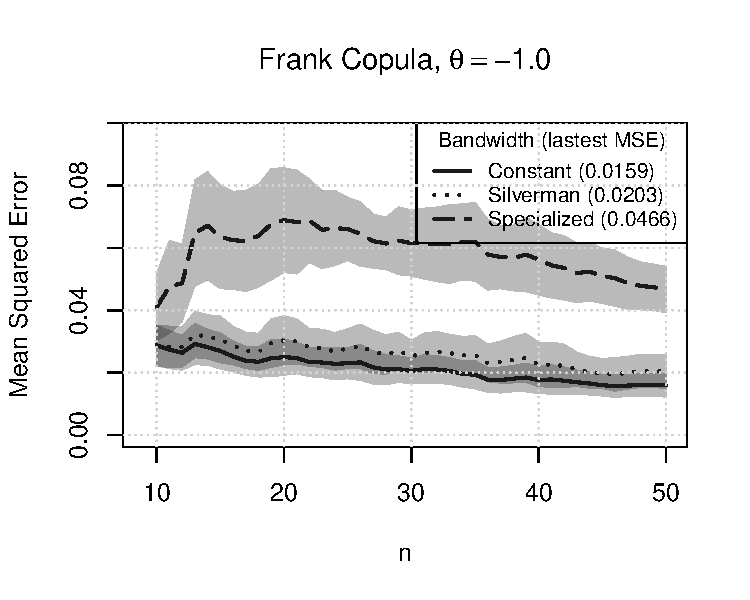
\includegraphics[width=0.31\linewidth]{plots/experiment_results/frank_1}
			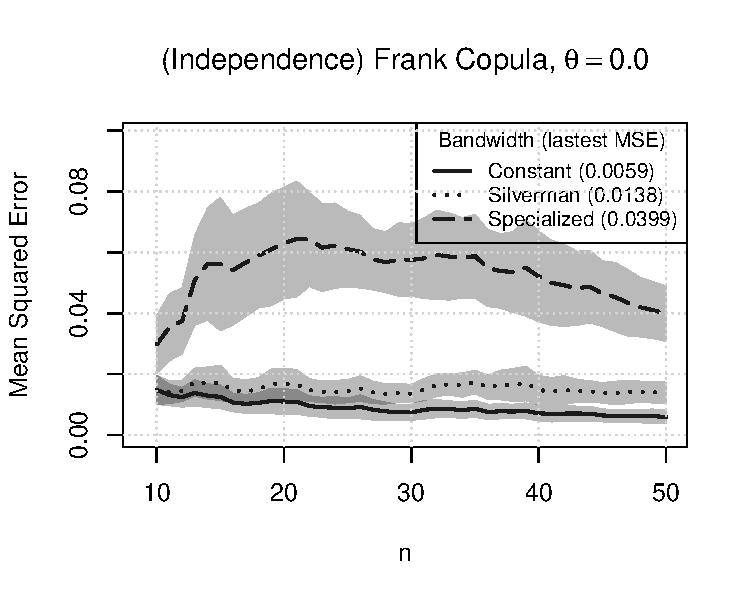
\includegraphics[width=0.31\linewidth]{plots/experiment_results/frank0}
			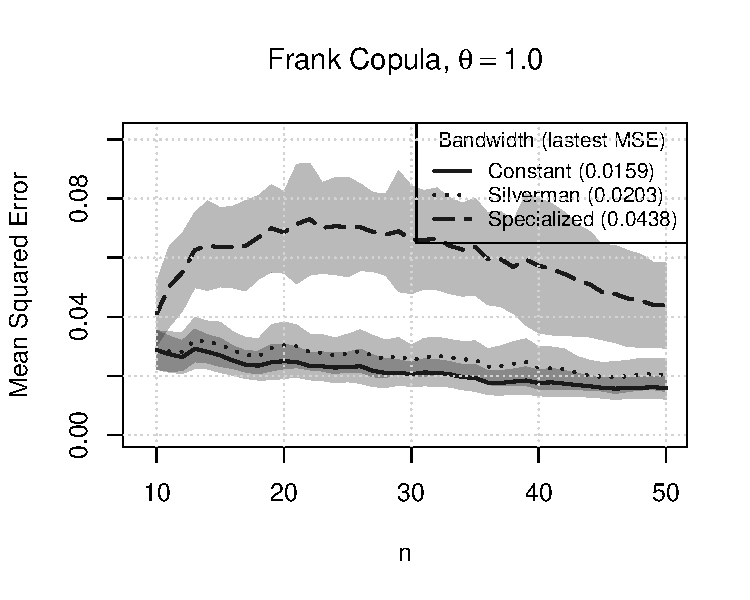
\includegraphics[width=0.31\linewidth]{plots/experiment_results/frank1}\\
			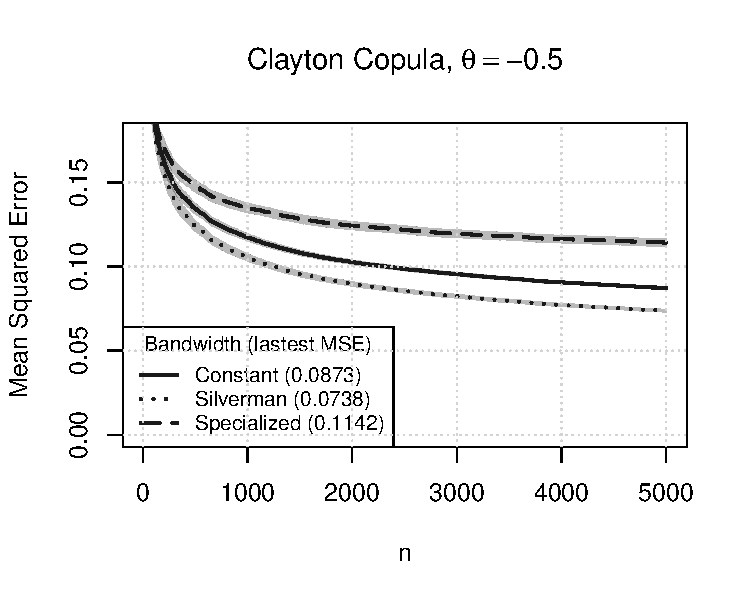
\includegraphics[width=0.31\linewidth]{plots/experiment_results/clayton_05}
			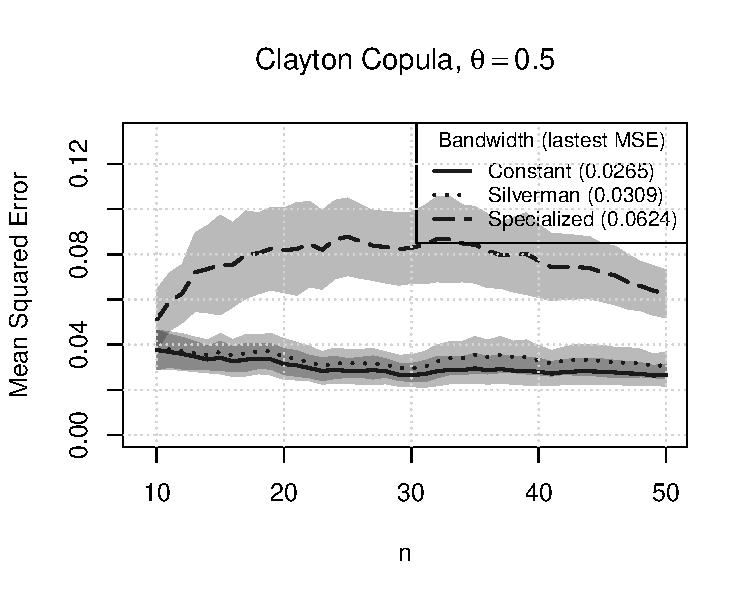
\includegraphics[width=0.31\linewidth]{plots/experiment_results/clayton05}
			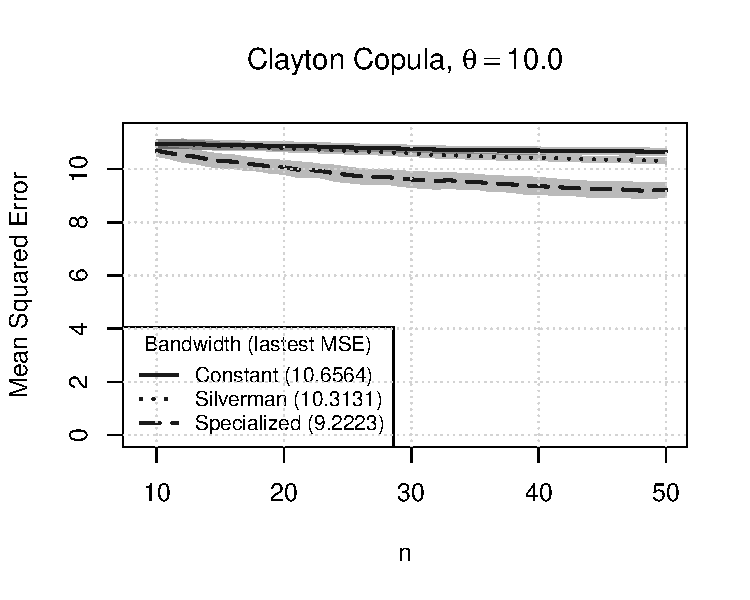
\includegraphics[width=0.31\linewidth]{plots/experiment_results/clayton10}\\
			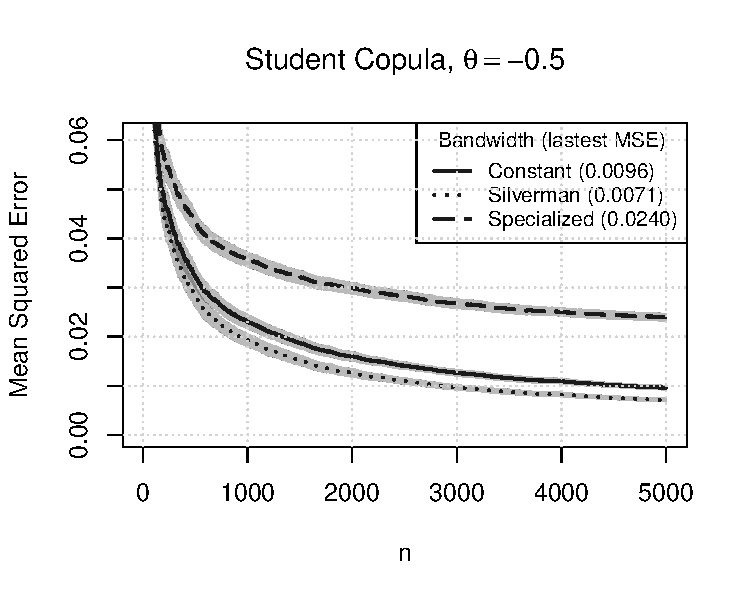
\includegraphics[width=0.31\linewidth]{plots/experiment_results/student_05}
			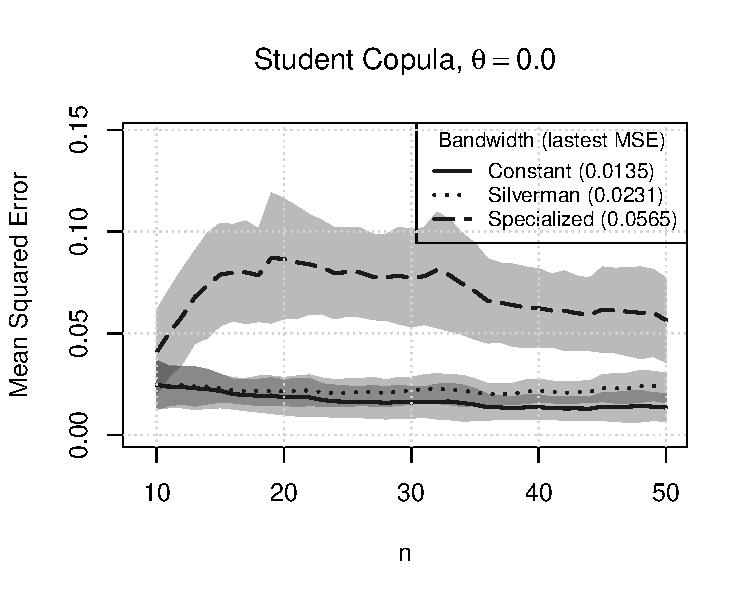
\includegraphics[width=0.31\linewidth]{plots/experiment_results/student0}
			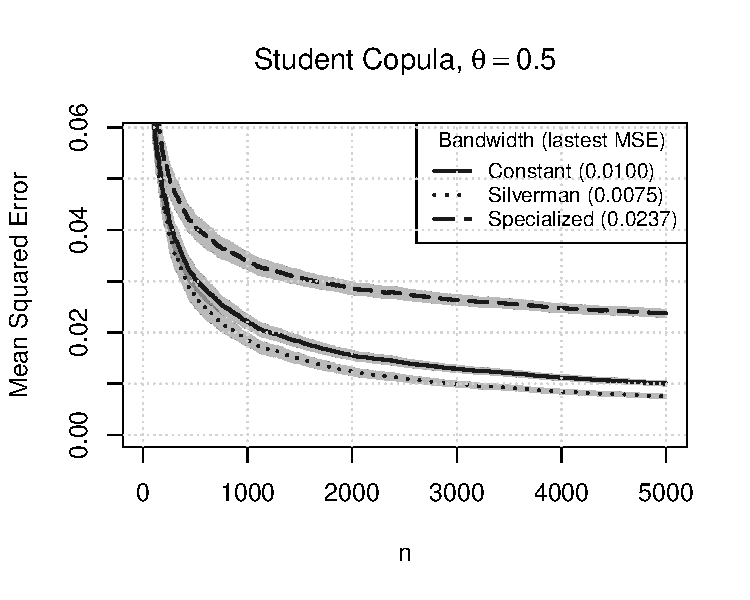
\includegraphics[width=0.31\linewidth]{plots/experiment_results/student05}
			\caption{Goodness of fit in numerical experiments for different types of copulas and different choices of bandwidth (\# of samples = 5K, \# of Monte Carlo simulations = 100, 95\,\% confidence interval).}
			%\caption{\textbf{??????????}}
			\label{fig:numerical_results}
		\end{figure}
	\end{landscape}
	
	\section{Conclusion}
	
	The contribution of this paper is two-fold. First of all, we introduced an algorithm of estimation of the multivariate joint density function using the smoothed non-parametric recursive estimator. Secondly, we successfully applied this estimator to the concept of copulas, joint distributions that enable to capture complex dependence structures among its variates. 
	
	The performance of the introduced algorithm for different experiment settings is successfully shown in numerical experiments. It is seen when a copula describes a reasonably complex, spiky, dependence structure the algorithms that use data-based bandwidths perform better, and, otherwise, data independent bandwidths achieve better results in more straightforward cases. The results of the experiments as well as other plots can be reproduced using the code that is available on \href{https://github.com/vdyashin/CopulaDensityEstimator}{\texttt{https://github.com/vdyashin/CopulaDensityEstimator}}.
	
	There is still research should be done in the area of automatic bandwidth selection as in most of the cases a simple data-independent bandwidth outperforms the more complex ones. In addition, it is also essential to find an application to this powerful analytical tool that is able to handle real-time parameter updates. We inclined to believe that the presented algorithms will be quite handy in estimating the dependence structure in conditions where the data-flow is ongoing.
	
	\section*{Acknowledgements}
	
	The author of this master thesis is grateful to his university Higher School of Economics for the provided opportunity to be an exchange student and be able to spend one semester in another campus where his scientific supervisor works and lives. The author also thanks the university staff including office managers Maria Neklyudova as well as Ekaterina Pavlova and Ilona Yakovleva for their support and responsiveness. Special gratitude to Felix Camirand (Ph.\,D.) from University of Melbourne who has provided an early version of his paper.
	
	I would also like to thank the uncountable number of contributors of \href{https://R-project.org/}{\textbf{R}} package and the creators of the \textbf{R} library \href{https://cran.r-project.org/web/packages/copula/copula.pdf}{\texttt{copula}}. The contributors of the \LaTeX~typesetting system are also gratefully acknowledged. 
	
	\nocite{R} \nocite{Rcopula1} \nocite{Rcopula2} \nocite{Rcopula3} \nocite{Rcopula4}
	
	\printbibliography
	\pagebreak
	\appendix
	\section{Types of Copulas}\label{sec:copula_types}
	
	There are two main classes of copulas: \textit{Archimedean} and \textit{Elliptical}. The Archimedean copulas are well-known for its simplicity in derivation and capability of capturing dependence structure quite well. The Elliptical copulas differ from the Archimedean ones in a way that they have an implicit expression that is based on the elliptical distribution families. Here we will follow the notation of Following the notations of \textcite{Hyrs2015}.
	
	\subsection{Archimedean copulas}
	
	The Archimedean copulas are defined through the \textit{generator} function. A generator is a function $ \psi: [0, \infty) \rightarrow [0, 1]$ which has the following properties:
	\begin{enumerate}
		\item $ \psi(0) = 1 $ and $ \lim_{t\rightarrow \infty}\psi(t) = 0 $;
		\item $ \psi(\cdot) $ is continuous;
		\item $ \psi(\cdot) $ is decreasing on $ [0, \infty) $ and strictly decreasing on $ \big[0, \inf\{t>0: \psi(t) = 0\}\big) $, given $ \psi(\emptyset) := 0 $
	\end{enumerate}
	
	$ d $-dimensional Archimedean copula is defined as follows
	\begin{align}
	C_\psi(u_1, \dots, u_d) := \psi\big(\psi^{-1}(u_1) + \dots + \psi^{-1}(u_d)\big),
	\end{align}
	where $ \psi(\cdot) $ denotes the generator and $ \psi^{-1}(\cdot) $ its inverse.
	
	The rationale behind the choice of this type for empirical applications is that by definition it may capture a wide range of dependence structure using different generators. In addition, it is quite easy to derive and estimate. 
	
	Next we define the three most popular Archimedean copulas: Frank, Clayton, and Gumbel. Also, we provide with definition of Independence copula. All of them has a simple functional form and one parameter $ \theta $ that depicts the dependency strength.
	
	\subsubsection{Independence Copula} The simples copula is the independence copula
	\begin{align}
	C(u_1, u_2) &= u_1 u_2 \\
	\psi(t) &= -\log(t) \\
	\psi^{-1}(t) &= -\exp[-t]
	\end{align}
	
	\subsubsection{Frank Copula} The bivariate Frank copula is defined as follows 
	\begin{align}
	C(u_1, u_2) &= - \frac{1}{\theta}\log\bigg(1 + \frac{(e^{-\theta u_1}-1)(e^{-\theta u_2}-1)}{e^{-\theta}-1}\bigg) \\
	\psi(t) &= -\frac{1}{\theta}\log\big(e^{-t}(e^{-\theta}-1)+1\big) \\
	\psi^{-1}(t) &= -\log\bigg(\frac{e^{-\theta t}-1}{e^{-\theta}-1}\bigg) \\
	\theta &\in \mathbb{R}\backslash \{0\}
	\end{align}
	
	\subsubsection{Gumbel Copula} We can define bivariate Gumbel copula
	\begin{align}
	C(u_1, u_2) &= \exp\bigg[-\Big((-\log(u_1))^\theta + \big(-\log(u_2)\big)^\theta\Big)^{1/\theta}\bigg] \\
	\psi(t) &= \exp\big[-t^{1/\theta}\big] \\
	\psi^{-1}(t) &= \big(-\log(t)\big)^\theta \\
	\theta &\in [1, \infty)
	\end{align}
	
	\subsubsection{Clayton Copula} And finally bivariate Clayton copula
	\begin{align}
	C(u_1, u_2) &= \max\big[u_1^{-\theta}+u_2^{-\theta}-1, 0\big]^{-1/\theta} \\
	\psi(t) &= (1+t)^{-1/\theta} \\
	\psi^{-1}(t) &= t^{-\theta}-1 \\
	\theta &\in [-1, \infty) \backslash \{0\}
	\end{align}
	
	\subsection{Elliptical Copulas}
	
	Compared with Archimedean copulas, elliptical copulas have only implicit formulation that follows from the Sklar's theorem. A $ d $-variate elliptical copula is defined in the following fashion
	\begin{align}
	C(u_1, u_2) := F_\Theta\big(F^{-1}(u_1), F^{-1}(u_2)\big),
	\end{align}
	where $ F_\Theta(\cdot) $ represents an elliptical distribution with covariance matrix $ \Theta $ and $ F^{-1}(\cdot) $ its inverse. The covariance matrix $ \Theta $ has $ (d^2 - d)/2 $ parameters to express the dependence structure. Therefore, this class of copulas may capture a wider range of dependencies in comparison with the Archimedean class \parencite{Hyrs2015}.
	
	There are two most popular types of copulas in the elliptical class: Normal (Gaussian) and Student copulas.
	
	\subsubsection{Student Copula} The bivariate Student copula that is governed by $ t $-distribution and defined as follows
	\begin{align}
	C(u_1, u_2) &= t_{\Theta, \eta} \big(t^{-1}_\eta(u_1), t^{-1}_\eta(u_2)\big) \\
	&= \int_{-\infty}^{t^{-1}_\eta(u_1)} \int_{-\infty}^{t^{-1}_\eta(u_2)} \frac{1}{2\pi\sqrt{1-\theta^2}}\bigg(1 + \frac{x^2 - 2\theta xy + y^2}{\eta(1-\theta^2)}\bigg)^{-(\eta + 2)/2} \text{d}x \text{d}y \\
	\theta &\in (-1, 1)
	\end{align}
	where $ t_{\Theta, \eta} $ is the multivariate $ t $-distribution and $ t^{-1}_\eta(u_1) $ is the quantile of the univariate $ t $-distribution with $ \eta $ degrees of freedom.
	
	\subsubsection{Gaussian Copula} Similarly, the bivariate Normal (Gaussian) copula is governed by Normal distribution
	\begin{align}
	C(u_1, u_2) &= \Phi_{\Theta}\big(\Phi^{-1}(u_1), \Phi^{-1}(u_2)\big) \\
	&= \int_{-\infty}^{\Phi^{-1}(u_1)} \int_{-\infty}^{\Phi^{-1}(u_2)} \frac{1}{2\pi\sqrt{1-\theta^2}}\exp\bigg[-\frac{x^2 - 2\theta xy + y^2}{2(1-\theta^2)}\bigg] \text{d}x \text{d}y \\
	\theta &\in (-1, 1)
	\end{align}
	
	The illustration of all of the described copulas can be seen in Figure~\ref{fig:copulas}. Also note that in most of the copulas there is exist a value of $ \theta $ such that the copula degenerate into independence copula (see. Frank and Normal copulas with $ \theta \approx 0 $).
	
	\begin{figure}
		\begin{flushright}
			\begin{tikzpicture}
			\draw [thick, <->, white] (0, 0) rectangle (3, 3);
			\node at (1.5, 1.5) {Frank Copula};
			\end{tikzpicture}
			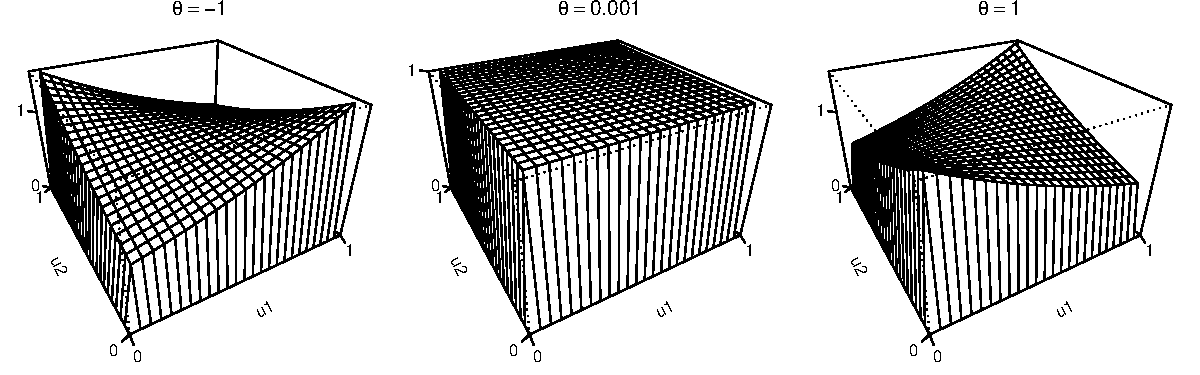
\includegraphics[width=0.77\linewidth]{plots/copulas/frank}\\
			\begin{tikzpicture}
			\draw [thick, <->, white] (0, 0) rectangle (3, 3);
			\node at (1.5, 1.5) {Gumbel Copula};
			\end{tikzpicture}
			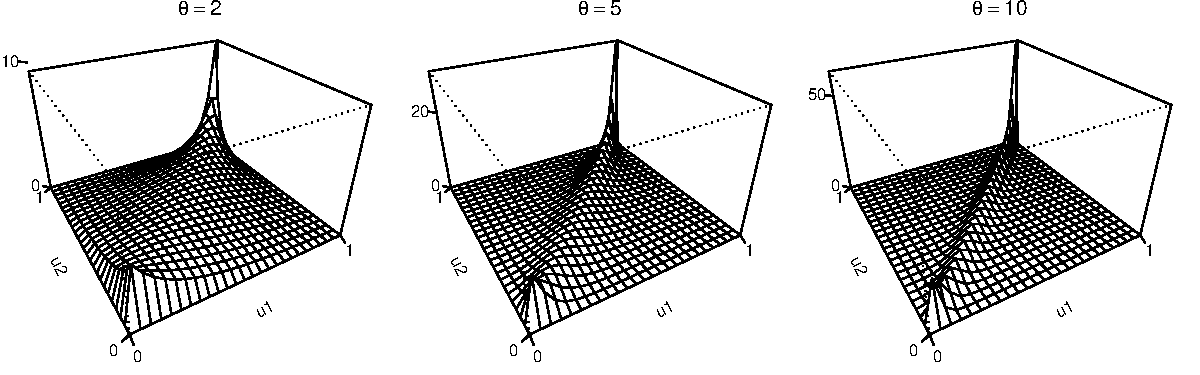
\includegraphics[width=0.77\linewidth]{plots/copulas/gumbel}\\
			\begin{tikzpicture}
			\draw [thick, <->, white] (0, 0) rectangle (3, 3);
			\node at (1.5, 1.5) {Clayton Copula};
			\end{tikzpicture}
			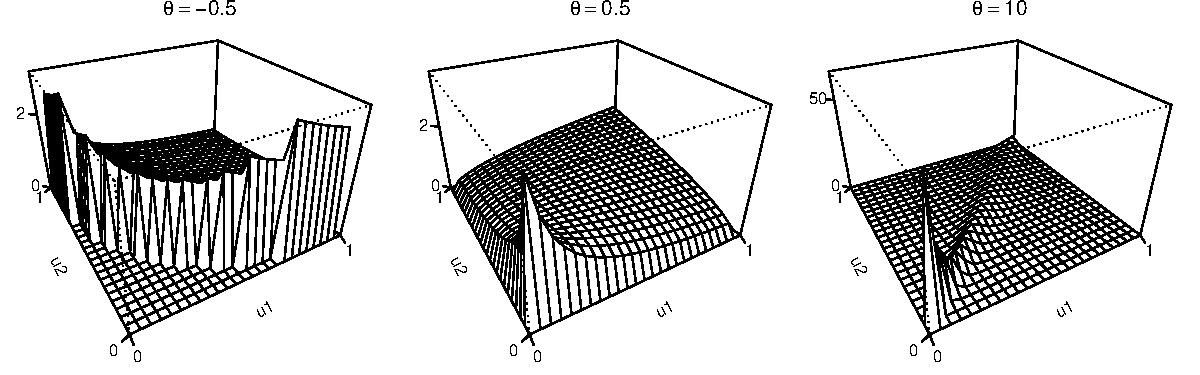
\includegraphics[width=0.77\linewidth]{plots/copulas/clayton}\\
			\begin{tikzpicture}
			\draw [thick, <->, white] (0, 0) rectangle (3, 3);
			\node at (1.5, 1.5) {Student Copula};
			\end{tikzpicture}
			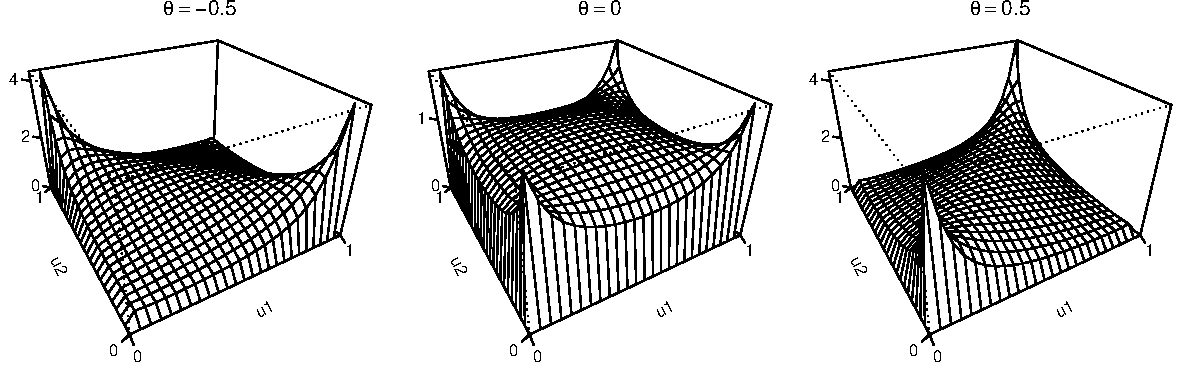
\includegraphics[width=0.77\linewidth]{plots/copulas/student}\\
			\begin{tikzpicture}
			\draw [thick, <->, white] (0, 0) rectangle (3, 3);
			\node at (1.5, 1.5) {Normal Copula};
			\end{tikzpicture}
			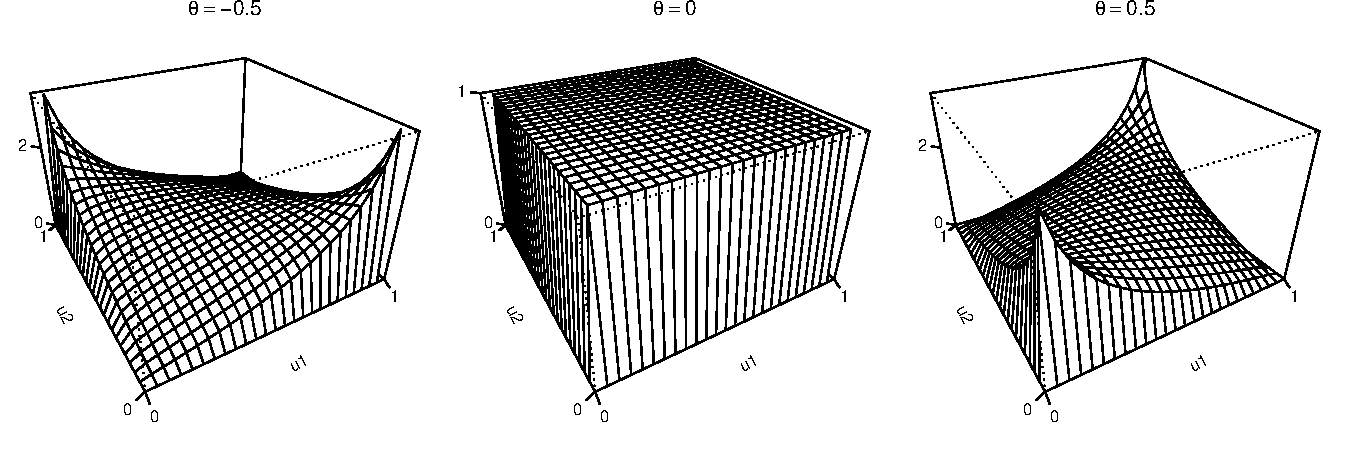
\includegraphics[width=0.77\linewidth]{plots/copulas/normal}\\
		\end{flushright}
		
		\caption{Different types of copulas with different parameter $ \theta $.}
		\label{fig:copulas}
	\end{figure}
	
	
	
	
	\section{Calculation of Bandwidth for the Joint Distribution}\label{sec:band_joint}
	
	Assume $ \alpha = 1 $, then $ C_\alpha = 1 $. A bandwidth can be presented as
	\begin{align}\label{eq:prod_band}
		b_n = C_h n^{-\theta}
	\end{align}
	
	So, let us start with the bias and variance formulas	that are obtained from Theorem~\ref{thm:asym_norm_joint}
	\begin{align}
		\text{Bias}\big(f_n^{\mathbf{u}}, f^{\mathbf{u}}\big) &= \frac{\eta b_n^2}{2(1-2\theta)} \sum_{j=1}^{d}f^{\mathbf{u}}_{(j,j)}\big(1+o(1)\big) \\
		\text{Variance}\big(f_n^{\mathbf{u}}\big) &= \frac{C_\beta^2\,\widetilde{\eta}^df^{\mathbf{u}}}{n^\beta(2-\beta)} \big(1+o(1)\big).
	\end{align}
	Then mean squared error is as follows
	\begin{align}
		\text{MSE}\big(f_n^{\mathbf{u}}\big) &= \text{Bias}^2\big(f_n^{\mathbf{u}}, f^{\mathbf{u}}\big) + \text{Variance}\big(f_n^{\mathbf{u}}\big) \\
		&= b^4_n \frac{\eta^2\!\cdot \big(\!\sum_{j=1}^{d}f^{\mathbf{u}}_{(j,j)}\big)^2} {4(1-2\theta)^2} + n^{-\beta} \frac{C_\beta^2\, \widetilde{\eta}^df^{\mathbf{u}}}{2-\beta}. \label{eq:mse_2}
	\end{align}
	Also, according to the Assumption~6 of Theorem~\ref{thm:asym_norm_joint} we put $ \beta=\alpha-d\theta=1-d\theta $. Thus, $ \beta < 2 $ and $ 1-d\theta < 2 $. Hence, the assumption is satisfied.
	
	Now, let us rewrite $ n^{-\beta} $
	\begin{align}
		n^{-\beta} = n^{-1+d\theta}= n^{-1}\big(n^{-\theta}\big)^{-d},
	\end{align}
	re-express \eqref{eq:prod_band} as 
	\begin{align}
		n^{-\theta} &= b_n C^{-1}_h \rightarrow \\
		n^{-\beta} &= n^{-1}\big(n^{-\theta}\big)^{-d}= n^{-1}\big(b_n C^{-1}_h\big)^{-d}. \label{eq:toPluginmse}
	\end{align}
	Then, we plug \eqref{eq:toPluginmse} into \eqref{eq:mse_2} and obtain the following
	\begin{align}
		\text{MSE}\big(f_n^{\mathbf{u}}\big) &= b^4_n \frac{\eta^2\!\cdot \big(\!\sum_{j=1}^{d}f^{\mathbf{u}}_{(j,j)}\big)^2} {4(1-2\theta)^2} + n^{-1}\big(b_n C^{-1}_h\big)^{-d} \frac{C_\beta^2\, \widetilde{\eta}^df^{\mathbf{u}}}{2-\beta} \\
		&= b^4_n \frac{\eta^2\!\cdot \big(\!\sum_{j=1}^{d}f^{\mathbf{u}}_{(j,j)}\big)^2} {4(1-2\theta)^2} + b_n^{-d} n^{-1} \frac{C_hC_\beta^2\, \widetilde{\eta}^df^{\mathbf{u}}}{2-\beta} \\
		&:= b^4_n\cdot A_1 + b_n^{-d} n^{-1} \cdot A_2
	\end{align}
	After the optimization of $ \text{MSE}\big(f_n^{\mathbf{u}}\big) $ on $ b_n $ we obtain
	\begin{align}
		b_n^{4+d} = \frac{d\cdot A_2}{4n\cdot A_1}.
	\end{align}
	If we rewrite bandwidth in the form of \eqref{eq:prod_band} we get
	\begin{align}
		b_n = \Bigg[\frac{d\cdot A_2}{4\cdot A_1}\Bigg]^{1/(d+4)}n^{-1/(d+4)}.\label{eq:band}
	\end{align}
	Thus, since $ b_n = C_h n^{-\theta} $, $ \theta = 1/(d+4) $. Also, recall $ \beta = 1-d\theta $, then $ \beta=4/(d+4) $. We also know from the Assumption~6 of the Theorem~\ref{thm:asym_norm_joint} that $ \beta \in \big(0, \min\{6\theta, 1\}\big) $. This is satisfied if we plug $ \beta $ in the brackets.
	
	Also note that
	\begin{align}
		\lim_{n \rightarrow \infty}n^{(\alpha+\beta)/2-1}h^{-d/2} &= C_\beta \\
		&= n^{(1+\beta)/2-1}\cdot\big(C_h\big)^{-d/2}\cdot \\
		&= C_h^{-d/2}\cdot n^{0} \\
		&\Rightarrow C_h^{-d/2} = C_\beta.
	\end{align}
	We plug $ \theta = 1/(d+4) $ into $ A_1 $ and $ A_2 $ which, in turn, we plug into \eqref{eq:band} and obtain the bandwidth coefficient $ C_h $ from \eqref{eq:prod_band}
	\begin{align}
		C_h = \Bigg[\frac{d\cdot C_h^d\cdot C_\beta^2\cdot \widetilde{\eta}^d \cdot f^{\mathbf{u}}\cdot (d+2)}{2\cdot \eta^2\cdot \big[\sum_{j=1}^{d}f^{\mathbf{u}}_{(j,j)}\big]^2(d+4)}\Bigg]^{1/(d+4)}.
	\end{align}
	We derived earlier that $ C_\beta=C^{-d/2}_h $. Using this in the last formula we may obtain the form of bandwidth that is presented in Section~\ref{sec:spec_bands}.
	
\end{document}

\section{Example of convergence}
An example of convergence of a empirical quantile to the ground truth quantile at point $ u = 0.5 $ ($ 50^\text{th} $ percentile) using the recursive online estimator provided in \eqref{eq:quantile_1}, \eqref{eq:quantile_2}, and \eqref{eq:quantile_3} given different $ \kappa $ for univariate case is shown in Figure~\ref{fig:quantile}. 

It is obvious that as $ n $ increases the squared error between the estimated quantile and ground truth tends to be converging to zero. Also, we may see that the optimal $ \kappa $ appears to lie within the range $ (0, 2] $: the lowest error achieved when $ \kappa $ is 1. In addition, the lower the $ \kappa $ the less stable convergence is. It could be easily explained by the fact that the lower the $ \kappa $ the more dramatic changes are made to the current estimation of quantile (see \eqref{eq:quantile_3}). Despite the fact that only the results of $ 50^\text{th} $ percentile are presented within the text, the same pattern and shape of the lines appear in other percentiles ranging from $ 10^\text{th} $ to $ 90^\text{th} $.

\begin{figure}
	\centering
	\includegraphics[width=0.7\linewidth]{plots/quantile}
	\caption{Recursive non-parametric estimation of $ 0.5 $ quantile of the univariate standard normal distribution (\# of samples = 10K, \# of Monte Carlo simulations = 500). }
	\label{fig:quantile}
\end{figure}

%% gamma
\begin{align}
f^{\mathbf{u}}_n &= \bigg(1 - \frac{1}{i}\bigg)f^{\mathbf{u}}_{i-1} + \frac{1}{i} W_{t_n}^{\mathbf{u}} \big(Q_{i-1}^{\mathbf{u}} - \mathbf{X}_n\big) \\
c_n &= \frac{f^{\mathbf{u}}_n}{f^{u_1}_{1,i} \dots  f^{u_d}_{d,i}} 
\end{align}
where $ W_{t_n}^{\mathbf{u}}(\mathbf{X}) = \prod_{j=1}^{d}K_{t_{i}}^{u_j}(\mathbf{X}_j) $. In addition, $ Q_{i-1}^{\mathbf{u}} $ are quantiles estimated at the given grid of points $ \mathbf{u} $, and $ \mathbf{X}_n $ is the current $ d $-dimensional data point.






%% MARGINAL DENSITY REMOVED
\subsubsection{Marginal Density Bandwidths}

Similarly, we may use Theorem~\ref{thm:asym_norm_marginal} in order to obtain formulas for bias and variance to calculate the mean squared error of our estimator $ f_{j,n}^{u_j} $
\begin{align}
\text{Bias}\big(f_{j,n}^{u_j}, f_j^{u_j}\big) &= \frac{R_1^{1/2}\cdot\big(f_j^{u_j}\big)''\eta}{2 - \lambda} \\
\text{Variance}\big(f_n^{\mathbf{u}}\big) &= \frac{f_j^{u_j}\,\widetilde{\eta}}{2-\lambda},
\end{align}
then, the mean squared error can be defined as follows
\begin{align}
\text{MSE}\big(f_{j,n}^{u_j}\big) &= \text{Bias}^2\big(f_{j,n}^{u_j}, f^{u_j}_j\big) + \text{Variance}\big(f_{j,n}^{u_j}\big) \\
&= n\cdot h^5_{j,n}\frac{\Big[\big(f_j^{u_j}\big)''\Big]^2\eta^2}{(2 - \lambda)^2} + \frac{f_j^{u_j}\,\widetilde{\eta}}{2-\lambda}.
\end{align}

Now in a similar way, the optimal bandwidth $ h_{j,n} $ for a marginal density $ f_{j,n}^{u_j} $ might be derived as
\begin{align}
h_{j,n} = \arg \min_{h_{j,n}} \big\{\text{MSE}\big(f_{j,n}^{u_j}\big)\big\} =  \Bigg[\frac{\widetilde{\eta}\cdot f_j^{u_j}\cdot(2-\lambda)}{4\cdot \big[\big(f_j^{u_j}\big)''\!\cdot\eta\big]^2}\Bigg]^{\frac{1}{5}} \cdot n^{-\frac{1}{5}}. \label{eq:bandwidth_marginal}
\end{align}

\begin{center}
	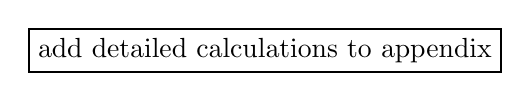
\begin{tikzpicture}
	\node[draw, thick] {add detailed calculations to appendix};
	\end{tikzpicture}
\end{center}

The presented bandwidth $ h_{j,n} $ is used to estimate the joint density introduced in \eqref{eq:quantile_2}. The proof of the \eqref{eq:bandwidth_marginal} can be found in Appendix~\ref{sec:band_marginals}.
